\documentclass{article}
\usepackage{amsmath, amssymb, ctex, graphicx}
\usepackage[margin=1in]{geometry}
\title{第2章-概率-所有习题}
\author{《深度学习基础》课程小组}
% \date{}

\begin{document}
\maketitle

\textbf{2.1} ($\star$) In the cancer screening example, we used a prior probability of cancer of $p(C = 1) = 0.01$. In reality, the prevalence of cancer is generally very much lower. Consider a situation in which $p(C = 1) = 0.001$, and recompute the probability of having cancer given a positive test $p(C = 1|T = 1)$. Intuitively, the result can appear surprising to many people since the test seems to have high accuracy and yet a positive test still leads to a low probability of having cancer.

\textbf{2.1} ($\star$) 在癌症筛查的例子中，我们使用了患癌的先前概率为$p(C = 1) = 0.01$。实际上，癌症的发病率通常要低得多。考虑一种情况，其中$p(C = 1) = 0.001$，并重新计算在检测呈阳性的情况下患有癌症的概率$p(C = 1|T = 1)$。直观上，这个结果可能会让许多人感到惊讶，因为该测试似乎具有很高的准确性，但阳性检测结果仍然导致患有癌症的概率很低。

\textbf{2.2} ($\star\star$) Deterministic numbers satisfy the property of \emph{transitivity}, so that if $x > y$ and $y > z$ then it follows that $x > z$. When we go to random numbers, however, this property need no longer apply. Figure 2.16 shows a set of four cubical dice that have been arranged in a cyclic order. Show that each of the four dice has a 2/3 probability of rolling a higher number than the previous die in the cycle. Such dice are known as \emph{non-transitive dice}, and the specific examples shown here are called \emph{Efron dice}.

\textbf{2.2} ($\star\star$) 确定性数字满足\emph{传递性}属性，因此如果$x > y$且$y > z$，则可以得出$x > z$。然而，当我们转向随机数时，此属性不再适用。图2.16展示了一组按循环顺序排列的四个立方体骰子。证明这四个骰子中的每一个都有2/3的概率掷出比循环中前一个骰子更高的数字。这样的骰子被称为\emph{非传递性骰子}，这里显示的具体例子被称为\emph{埃夫龙骰子}。

\begin{figure}[ht]
    \centering
    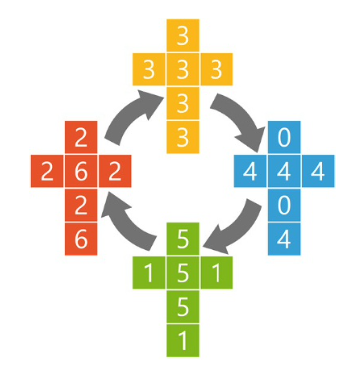
\includegraphics[height=5cm]{efron_dice.png}
    \caption{An example of non-transitive cubical dice}
    \label{fig:efron_dice}
\end{figure}

An example of non-transitive cubical dice, in which each die has been 'flattened' to reveal the numbers on each of the faces. The dice have been arranged in a cycle, such that each die has a 2/3 probability of rolling a higher number than the previous die in the cycle. 

非传递性立方体骰子的一个例子，其中每个骰子都被“压平”以显示每个面上的数字。这些骰子被排列成一个循环，使得每个骰子有2/3的概率掷出比循环中前一个骰子更高的数字。

\textbf{2.3} ($\star$) Consider a variable $\mathbf{y}$ given by the sum of two independent random variables $\mathbf{y} = \mathbf{u} + \mathbf{v}$ where $\mathbf{u} \sim p_{\mathbf{u}}(\mathbf{u})$ and $\mathbf{v} \sim p_{\mathbf{v}}(\mathbf{v})$. Show that the distribution $p_{\mathbf{y}}(\mathbf{y})$ is given by
\begin{equation}
p(\mathbf{y}) = \int p_{\mathbf{u}}(\mathbf{u})p_{\mathbf{v}}(\mathbf{y} - \mathbf{u}) \,\mathrm{d}\mathbf{u}. \tag{2.119}
\end{equation}
This is known as the \emph{convolution} of $p_{\mathbf{u}}(\mathbf{u})$ and $p_{\mathbf{v}}(\mathbf{v})$.

\textbf{2.3} ($\star$) 考虑一个变量$\mathbf{y}$，它由两个独立随机变量的和给出，即$\mathbf{y} = \mathbf{u} + \mathbf{v}$，其中$\mathbf{u} \sim p_{\mathbf{u}}(\mathbf{u})$且$\mathbf{v} \sim p_{\mathbf{v}}(\mathbf{v})$。证明分布$p_{\mathbf{y}}(\mathbf{y})$由下式给出：
\begin{equation}
p(\mathbf{y}) = \int p_{\mathbf{u}}(\mathbf{u})p_{\mathbf{v}}(\mathbf{y} - \mathbf{u}) \,\mathrm{d}\mathbf{u}. \tag{2.119}
\end{equation}
这被称为$p_{\mathbf{u}}(\mathbf{u})$和$p_{\mathbf{v}}(\mathbf{v})$的\emph{卷积}。

\textbf{2.4} ($\star\star$) Verify that the uniform distribution (2.33) is correctly normalized, and find expressions for its mean and variance.

\textbf{2.4} ($\star\star$) 验证均匀分布(2.33)是否正确归一化，并找出其均值和方差的表达式。

\textbf{2.5} ($\star\star$) Verify that the exponential distribution (2.34) and the Laplace distribution (2.35) are correctly normalized.

\textbf{2.5} ($\star\star$) 验证指数分布(2.34)和拉普拉斯分布(2.35)是否正确归一化。

\textbf{2.6} ($\star$) Using the properties of the Dirac delta function, show that the empirical density (2.37) is correctly normalized.

\textbf{2.6} ($\star$) 利用狄拉克$\delta$函数的性质，证明经验密度(2.37)是正确归一化的。

\textbf{2.7} ($\star$) By making use of the empirical density (2.37), show that the expectation given by (2.39) can be approximated by a sum over a finite set of samples drawn from the density in the form (2.40).

\textbf{2.7} ($\star$) 通过利用经验密度(2.37)，证明由(2.39)给出的期望可以通过对从该密度中抽取的一组有限样本求和来近似，形式如(2.40)所示。

\textbf{2.8} ($\star$) Using the definition (2.44), show that $\text{var}[f(x)]$ satisfies (2.45).

\textbf{2.8} ($\star$) 使用定义(2.44)，证明$\text{var}[f(x)]$满足(2.45)。

\textbf{2.9} ($\star$) Show that if two variables $x$ and $y$ are independent, then their covariance is zero.

\textbf{2.9} ($\star$) 证明如果两个变量$x$和$y$是独立的，那么它们的协方差为零。

\textbf{2.10} ($\star$) Suppose that the two variables $x$ and $z$ are statistically independent. Show that the mean and variance of their sum satisfies
\begin{align}
\mathbb{E}[x + z] &= \mathbb{E}[x] + \mathbb{E}[z] \tag{2.120} \\
\text{var}[x + z] &= \text{var}[x] + \text{var}[z]. \tag{2.121}
\end{align}

\textbf{2.10} ($\star$) 假设两个变量$x$和$z$是统计独立的。证明它们之和的均值和方差满足
\begin{align}
\mathbb{E}[x + z] &= \mathbb{E}[x] + \mathbb{E}[z] \tag{2.120} \\
\text{var}[x + z] &= \text{var}[x] + \text{var}[z]. \tag{2.121}
\end{align}

\textbf{2.11} ($\star$) Consider two variables $x$ and $y$ with joint distribution $p(x, y)$. Prove the following two results:
\begin{align}
\mathbb{E}[x] &= \mathbb{E}_y [\mathbb{E}_x[x|y]] \tag{2.122} \\
\text{var}[x] &= \mathbb{E}_y [\text{var}_x[x|y]] + \text{var}_y [\mathbb{E}_x[x|y]]. \tag{2.123}
\end{align}
Here $\mathbb{E}_x[x|y]$ denotes the expectation of $x$ under the conditional distribution $p(x|y)$, with a similar notation for the conditional variance.

\textbf{2.11} ($\star$) 考虑两个具有联合分布$p(x, y)$的变量$x$和$y$。证明以下两个结果：
\begin{align}
\mathbb{E}[x] &= \mathbb{E}_y [\mathbb{E}_x[x|y]] \tag{2.122} \\
\text{var}[x] &= \mathbb{E}_y [\text{var}_x[x|y]] + \text{var}_y [\mathbb{E}_x[x|y]]. \tag{2.123}
\end{align}
这里$\mathbb{E}_x[x|y]$表示在条件分布$p(x|y)$下$x$的期望，条件方差也有类似的记号。

\textbf{2.12} ($\star\star\star$) In this exercise, we prove the normalization condition (2.51) for the univariate Gaussian. To do this consider, the integral
\begin{equation}
I = \int_{-\infty}^{\infty} \exp \left( -\frac{1}{2\sigma^2}x^2 \right) \,\mathrm{d}x \tag{2.124}
\end{equation}
which we can evaluate by first writing its square in the form
\begin{equation}
I^2 = \int_{-\infty}^{\infty} \int_{-\infty}^{\infty} \exp \left( -\frac{1}{2\sigma^2}x^2 - \frac{1}{2\sigma^2}y^2 \right) \,\mathrm{d}x \,\mathrm{d}y. \tag{2.125}
\end{equation}
Now make the transformation from Cartesian coordinates $(x, y)$ to polar coordinates $(r, \theta)$ and then substitute $u = r^2$. Show that, by performing the integrals over $\theta$ and $u$ and then taking the square root of both sides, we obtain
\begin{equation}
I = \left( 2\pi\sigma^2 \right)^{1/2}. \tag{2.126}
\end{equation}
Finally, use this result to show that the Gaussian distribution $\mathcal{N}(x|\mu, \sigma^2)$ is normalized.

\textbf{2.12} ($\star\star\star$) 在本练习中，我们证明单变量高斯分布的归一化条件(2.51)。为此，考虑积分
\begin{equation}
I = \int_{-\infty}^{\infty} \exp \left( -\frac{1}{2\sigma^2}x^2 \right) \,\mathrm{d}x \tag{2.124}
\end{equation}
我们可以通过首先将其平方写成如下形式来计算它
\begin{equation}
I^2 = \int_{-\infty}^{\infty} \int_{-\infty}^{\infty} \exp \left( -\frac{1}{2\sigma^2}x^2 - \frac{1}{2\sigma^2}y^2 \right) \,\mathrm{d}x \,\mathrm{d}y. \tag{2.125}
\end{equation}
现在进行从笛卡尔坐标$(x, y)$到极坐标$(r, \theta)$的变换，然后代入$u = r^2$。证明通过对$\theta$和$u$进行积分，然后对两边取平方根，我们得到
\begin{equation}
I = \left( 2\pi\sigma^2 \right)^{1/2}. \tag{2.126}
\end{equation}
最后，利用这个结果证明高斯分布$\mathcal{N}(x|\mu, \sigma^2)$是归一化的。

\textbf{2.13} ($\star\star$) By using a change of variables, verify that the univariate Gaussian distribution given by (2.49) satisfies (2.52). Next, by differentiating both sides of the normalization condition
\begin{equation}
\int_{-\infty}^{\infty} \mathcal{N}\left(x | \mu, \sigma^{2}\right) \mathrm{d} x=1
\tag{2.127}
\end{equation}
with respect to $\sigma^{2}$, verify that the Gaussian satisfies (2.53). Finally, show that (2.54) holds.

\textbf{2.13} ($\star\star$) 通过变量代换，验证由(2.49)给出的单变量高斯分布满足(2.52)。接下来，通过对归一化条件
\begin{equation}
\int_{-\infty}^{\infty} \mathcal{N}\left(x | \mu, \sigma^{2}\right) \mathrm{d} x=1
\tag{2.127}
\end{equation}
的两边关于$\sigma^{2}$求导，验证高斯分布满足(2.53)。最后，证明(2.54)成立。

\textbf{2.14} ($\star$) Show that the mode (i.e., the maximum) of the Gaussian distribution (2.49) is given by $\mu$.

\textbf{2.14} ($\star$) 证明高斯分布(2.49)的众数（即最大值）由$\mu$给出。

\textbf{2.15} ($\star$) By setting the derivatives of the log likelihood function (2.56) with respect to $\mu$ and $\sigma^{2}$ equal to zero, verify the results (2.57) and (2.58).

\textbf{2.15} ($\star$) 通过对数似然函数(2.56)关于$\mu$和$\sigma^{2}$的导数设为零，验证结果(2.57)和(2.58)。

\textbf{2.16} ($\star\star$) Using the results (2.52) and (2.53), show that
\begin{equation}
\mathbb{E}\left[x_{n} x_{m}\right]=\mu^{2}+I_{n m} \sigma^{2}
\tag{2.128}
\end{equation}
where $x_{n}$ and $x_{m}$ denote data points sampled from a Gaussian distribution with mean $\mu$ and variance $\sigma^{2}$ and $I_{nm}$ satisfies $I_{nm}=1$ if $n=m$ and $I_{nm}=0$ otherwise. Hence prove the results (2.59) and (2.60).

\textbf{2.16} ($\star\star$) 利用结果(2.52)和(2.53)，证明
\begin{equation}
\mathbb{E}\left[x_{n} x_{m}\right]=\mu^{2}+I_{n m} \sigma^{2}
\tag{2.128}
\end{equation}
其中$x_{n}$和$x_{m}$表示从均值为$\mu$、方差为$\sigma^{2}$的高斯分布中采样的数据点，并且$I_{nm}$在$n=m$时满足$I_{nm}=1$，否则$I_{nm}=0$。从而证明结果(2.59)和(2.60)。

\textbf{2.17} ($\star\star$) Using the definition (2.61), prove the result (2.62) which shows that the expectation of the variance estimator for a Gaussian distribution based on the true mean is given by the true variance $\sigma^{2}$.

\textbf{2.17} ($\star\star$) 使用定义(2.61)，证明结果(2.62)，该结果表明基于真实均值的高斯分布的方差估计量的期望由真实方差$\sigma^{2}$给出。

\textbf{2.18} ($\star$) Show that maximizing (2.66) with respect to $\sigma^{2}$ gives the result (2.68).

\textbf{2.18} ($\star$) 证明关于$\sigma^{2}$最大化(2.66)会得到结果(2.68)。

\textbf{2.19} ($\star\star$) Use the transformation property (2.71) of a probability density under a change of variable to show that any density $p(y)$ can be obtained from a fixed density $q(x)$ that is everywhere non-zero by making a nonlinear change of variable $y=f(x)$ in which $f(x)$ is a monotonic function so that $0 \leqslant f^{\prime}(x)<\infty$. Write down the differential equation satisfied by $f(x)$ and draw a diagram illustrating the transformation of the density.

\textbf{2.19} ($\star\star$) 利用概率密度在变量变换下的变换性质(2.71)，证明任何密度$p(y)$都可以通过对一个处处非零的固定密度$q(x)$进行非线性变量变换$y=f(x)$来获得，其中$f(x)$是一个单调函数，使得$0 \leqslant f^{\prime}(x)<\infty$。写出$f(x)$所满足的微分方程，并绘制一个图示来说明密度的变换。

\textbf{2.20} ($\star$) Evaluate the elements of the Jacobian matrix for the transformation defined by (2.78) and (2.79).

\textbf{2.20} ($\star$) 计算由(2.78)和(2.79)定义的变换的雅可比矩阵的元素。

\textbf{2.21} ($\star$) In Section 2.5, we introduced the idea of entropy $h(x)$ as the information gained on observing the value of a random variable $x$ having distribution $p(x)$. We saw that, for independent variables $x$ and $y$ for which $p(x, y)=p(x) p(y)$, the entropy functions are additive, so that $h(x, y)=h(x)+h(y)$. In this exercise, we derive the relation between $h$ and $p$ in the form of a function $h(p)$. First show that $h\left(p^{2}\right)=2 h(p)$ and, hence, by induction that $h\left(p^{n}\right)=n h(p)$ where $n$ is a positive integer. Hence, show that $h\left(p^{n / m}\right)=(n / m) h(p)$ where $m$ is also a positive integer. This implies that $h\left(p^{x}\right)=x h(p)$ where $x$ is a positive rational number and, hence, by continuity when it is a positive real number. Finally, show that this implies $h(p)$ must take the form $h(p) \propto \ln p$.

\textbf{2.21} ($\star$) 在2.5节中，我们引入了熵$h(x)$的概念，将其定义为观察具有分布$p(x)$的随机变量$x$的值所获得的信息。我们看到，对于满足$p(x, y)=p(x) p(y)$的独立变量$x$和$y$，熵函数是可加的，即$h(x, y)=h(x)+h(y)$。在本练习中，我们以函数$h(p)$的形式推导$h$和$p$之间的关系。首先证明$h\left(p^{2}\right)=2 h(p)$，因此，通过归纳法可得$h\left(p^{n}\right)=n h(p)$，其中$n$是正整数。由此，证明$h\left(p^{n / m}\right)=(n / m) h(p)$，其中$m$也是正整数。这意味着$h\left(p^{x}\right)=x h(p)$，其中$x$是正有理数，并且根据连续性，当它是正实数时也成立。最后，证明这蕴含着$h(p)$必须采取$h(p) \propto \ln p$的形式。

\textbf{2.22} ($\star$) Use a Lagrange multiplier to show that maximization of the entropy (2.86) for a discrete variable gives a distribution in which all of the probabilities $p\left(x_{i}\right)$ are equal and that the corresponding value of the entropy is then $\ln M$.

\textbf{2.22} ($\star$) 使用拉格朗日乘子法证明，对于一个离散变量，最大化熵(2.86)会得到一个所有概率$p\left(x_{i}\right)$都相等的分布，并且相应的熵值为$\ln M$。

\textbf{2.23} ($\star$) Consider an $M$-state discrete random variable $x$, and use Jensen's inequality in the form (2.102) to show that the entropy of its distribution $p(x)$ satisfies $\mathrm{H}[x] \leqslant \ln M$.

\textbf{2.23} ($\star$) 考虑一个$M$状态的离散随机变量$x$，并使用形式为(2.102)的琴生不等式，证明其分布$p(x)$的熵满足$\mathrm{H}[x] \leqslant \ln M$。

\textbf{2.24} ($\star\star$) Use the calculus of variations to show that the stationary point of the functional (2.96) is given by (2.97). Then use the constraints (2.93), (2.94), and (2.95) to eliminate the Lagrange multipliers and, hence, show that the maximum entropy solution is given by the Gaussian (2.98).

\textbf{2.24} ($\star\star$) 使用变分法证明泛函(2.96)的驻点由(2.97)给出。然后利用约束条件(2.93)、(2.94)和(2.95)消去拉格朗日乘子，从而证明最大熵解由高斯分布(2.98)给出。

\textbf{2.25} ($\star$) Use the results (2.94) and (2.95) to show that the entropy of the univariate Gaussian (2.98) is given by (2.99).

\textbf{2.25} ($\star$) 利用结果(2.94)和(2.95)证明单变量高斯分布(2.98)的熵由(2.99)给出。

\textbf{2.26} ($\star\star$) Suppose that $p(\mathbf{x})$ is some fixed distribution and that we wish to approximate it using a Gaussian distribution $q(\mathbf{x})=\mathcal{N}(\mathbf{x} | \boldsymbol{\mu}, \boldsymbol{\Sigma})$. By writing down the form of the Kullback-Leibler divergence $\mathrm{KL}(p \| q)$ for a Gaussian $q(\mathbf{x})$ and then differentiating, show that minimization of $\mathrm{KL}(p \| q)$ with respect to $\boldsymbol{\mu}$ and $\boldsymbol{\Sigma}$ leads to the result that $\boldsymbol{\mu}$ is given by the expectation of $\mathbf{x}$ under $p(\mathbf{x})$ and that $\boldsymbol{\Sigma}$ is given by the covariance.

\textbf{2.26} ($\star\star$) 假设$p(\mathbf{x})$是某个固定的分布，我们希望用一个高斯分布$q(\mathbf{x})=\mathcal{N}(\mathbf{x} | \boldsymbol{\mu}, \boldsymbol{\Sigma})$来近似它。通过写出高斯分布$q(\mathbf{x})$的Kullback-Leibler散度$\mathrm{KL}(p \| q)$的形式然后求导，证明关于$\boldsymbol{\mu}$和$\boldsymbol{\Sigma}$最小化$\mathrm{KL}(p \| q)$会导致这样的结果：$\boldsymbol{\mu}$由$\mathbf{x}$在$p(\mathbf{x})$下的期望给出，而$\boldsymbol{\Sigma}$由协方差给出。

\textbf{2.27} ($\star\star$) Evaluate the Kullback-Leibler divergence (2.100) between the two Gaussians $p(x)=\mathcal{N}\left(x | \mu, \sigma^{2}\right)$ and $q(x)=\mathcal{N}\left(x | m, s^{2}\right)$.

\textbf{2.27} ($\star\star$) 计算两个高斯分布$p(x)=\mathcal{N}\left(x | \mu, \sigma^{2}\right)$和$q(x)=\mathcal{N}\left(x | m, s^{2}\right)$之间的Kullback-Leibler散度(2.100)。

\textbf{2.28} ($\star\star$) The alpha family of divergences is defined by
\begin{equation}
\mathrm{D}_{\alpha}(p \| q)=\frac{4}{1-\alpha^{2}}\left(1-\int p(x)^{(1+\alpha) / 2} q(x)^{(1-\alpha) / 2} \mathrm{~d} x\right)
\tag{2.129}
\end{equation}
where $-\infty<\alpha<\infty$ is a continuous parameter. Show that the Kullback-Leibler divergence $\mathrm{KL}(p \| q)$ corresponds to $\alpha \rightarrow 1$. This can be done by writing $p^{\epsilon}=\exp (\epsilon \ln p)=1+\epsilon \ln p+O\left(\epsilon^{2}\right)$ and then taking $\epsilon \rightarrow 0$. Similarly, show that $\mathrm{KL}(q \| p)$ corresponds to $\alpha \rightarrow-1$.

\textbf{2.28} ($\star\star$) $\alpha$族散度定义为
\begin{equation}
\mathrm{D}_{\alpha}(p \| q)=\frac{4}{1-\alpha^{2}}\left(1-\int p(x)^{(1+\alpha) / 2} q(x)^{(1-\alpha) / 2} \mathrm{~d} x\right)
\tag{2.129}
\end{equation}
其中$-\infty<\alpha<\infty$是一个连续参数。证明Kullback-Leibler散度$\mathrm{KL}(p \| q)$对应于$\alpha \rightarrow 1$。这可以通过写成$p^{\epsilon}=\exp (\epsilon \ln p)=1+\epsilon \ln p+O\left(\epsilon^{2}\right)$然后令$\epsilon \rightarrow 0$来完成。同样地，证明$\mathrm{KL}(q \| p)$对应于$\alpha \rightarrow-1$。

\textbf{2.29} ($\star\star$) Consider two variables $\mathbf{x}$ and $\mathbf{y}$ having joint distribution $p(\mathbf{x}, \mathbf{y})$. Show that the differential entropy of this pair of variables satisfies
\begin{equation}
\mathrm{H}[\mathbf{x}, \mathbf{y}] \leqslant \mathrm{H}[\mathbf{x}]+\mathrm{H}[\mathbf{y}]
\tag{2.130}
\end{equation}
with equality if, and only if, $\mathbf{x}$ and $\mathbf{y}$ are statistically independent.

\textbf{2.29} ($\star\star$) 考虑两个具有联合分布$p(\mathbf{x}, \mathbf{y})$的变量$\mathbf{x}$和$\mathbf{y}$。证明这对变量的微分熵满足
\begin{equation}
\mathrm{H}[\mathbf{x}, \mathbf{y}] \leqslant \mathrm{H}[\mathbf{x}]+\mathrm{H}[\mathbf{y}]
\tag{2.130}
\end{equation}
当且仅当$\mathbf{x}$和$\mathbf{y}$统计独立时取等号。

\textbf{2.30} ($\star$) Consider a vector $\mathbf{x}$ of continuous variables with distribution $p(\mathbf{x})$ and corresponding entropy $\mathrm{H}[\mathbf{x}]$. Suppose that we make a non-singular linear transformation of $\mathbf{x}$ to obtain a new variable $\mathbf{y}=\mathbf{A} \mathbf{x}$. Show that the corresponding entropy is given by $\mathrm{H}[\mathbf{y}]=\mathrm{H}[\mathbf{x}]+\ln \operatorname{det} \mathbf{A}$ where $\operatorname{det} \mathbf{A}$ denotes the determinant of $\mathbf{A}$.

\textbf{2.30} ($\star$) 考虑一个具有分布$p(\mathbf{x})$和相应熵$\mathrm{H}[\mathbf{x}]$的连续变量向量$\mathbf{x}$。假设我们对$\mathbf{x}$做一个非奇异线性变换以获得一个新变量$\mathbf{y}=\mathbf{A} \mathbf{x}$。证明相应的熵由$\mathrm{H}[\mathbf{y}]=\mathrm{H}[\mathbf{x}]+\ln \operatorname{det} \mathbf{A}$给出，其中$\operatorname{det} \mathbf{A}$表示$\mathbf{A}$的行列式。

\textbf{2.31} ($\star\star$) Suppose that the conditional entropy $\mathrm{H}[y | x]$ between two discrete random variables $x$ and $y$ is zero. Show that, for all values of $x$ such that $p(x)>0$, the variable $y$ must be a function of $x$. In other words, for each $x$ there is only one value of $y$ such that $p(y | x) \neq 0$.

\textbf{2.31} ($\star\star$) 假设两个离散随机变量$x$和$y$之间的条件熵$\mathrm{H}[y | x]$为零。证明对于所有满足$p(x)>0$的$x$值，变量$y$必须是$x$的函数。换句话说，对于每个$x$，只有一个$y$值使得$p(y | x) \neq 0$。


\textbf{2.32} ($\star$) A strictly convex function is defined as one for which every chord lies above the function. Show that this is equivalent to the condition that the second derivative of the function is positive.

\textbf{2.32} ($\star$) 严格凸函数被定义为任意弦都位于函数图像上方的函数。证明这等价于该函数的二阶导数为正的条件。

\textbf{2.33} ($\star\star$) Using proof by induction, show that the inequality (2.101) for convex functions implies the result (2.102).

\textbf{2.33} ($\star\star$) 使用数学归纳法证明，关于凸函数的不等式(2.101)可以推出结果(2.102)。

\textbf{2.34} ($\star$) Show that, up to an additive constant, the Kullback–Leibler divergence (2.100) between the empirical distribution (2.37) and a model distribution $q(\mathbf{x}|\boldsymbol{\theta})$ is equal to the negative log likelihood function.

\textbf{2.34} ($\star$) 证明，除了一个相加的常数外，经验分布(2.37)与模型分布$q(\mathbf{x}|\boldsymbol{\theta})$之间的Kullback-Leibler散度(2.100)等于负对数似然函数。

\textbf{2.35} ($\star$) Using the definition (2.107) together with the product rule of probability, prove the result (2.108).

\textbf{2.35} ($\star$) 利用定义(2.107)以及概率的乘积法则，证明结果(2.108)。

\textbf{2.36} ($\star\star\star$) Consider two binary variables $x$ and $y$ having the joint distribution given by
\[
\begin{array}{c|cc}
 & \multicolumn{2}{c}{y} \\
x & 0 & 1 \\
\hline
0 & 1/3 & 1/3 \\
1 & 0 & 1/3 \\
\end{array}
\]
Evaluate the following quantities:
\begin{itemize}
    \item[(a)] $\mathrm{H}[x]$
    \item[(b)] $\mathrm{H}[y]$
    \item[(c)] $\mathrm{H}[y|x]$
    \item[(d)] $\mathrm{H}[x|y]$
    \item[(e)] $\mathrm{H}[x, y]$
    \item[(f)] $\mathrm{I}[x, y]$.
\end{itemize}
Draw a Venn diagram to show the relationship between these various quantities.

\textbf{2.36} ($\star\star\star$) 考虑两个具有如下联合分布的二元变量$x$和$y$：
\[
\begin{array}{c|cc}
 & \multicolumn{2}{c}{y} \\
x & 0 & 1 \\
\hline
0 & 1/3 & 1/3 \\
1 & 0 & 1/3 \\
\end{array}
\]
计算以下量：
\begin{itemize}
    \item[(a)] $\mathrm{H}[x]$
    \item[(b)] $\mathrm{H}[y]$
    \item[(c)] $\mathrm{H}[y|x]$
    \item[(d)] $\mathrm{H}[x|y]$
    \item[(e)] $\mathrm{H}[x, y]$
    \item[(f)] $\mathrm{I}[x, y]$.
\end{itemize}
绘制一个维恩图来展示这些不同量之间的关系。

\textbf{2.37} ($\star$) By applying Jensen’s inequality (2.102) with $f(x) = \ln x$, show that the arithmetic mean of a set of real numbers is never less than their geometrical mean.

\textbf{2.37} ($\star$) 通过对$f(x) = \ln x$应用琴生不等式(2.102)，证明一组实数的算术平均值永远不会小于它们的几何平均值。

\textbf{2.38} ($\star$) Using the sum and product rules of probability, show that the mutual information $I(\mathbf{x}, \mathbf{y})$ satisfies the relation (2.110).

\textbf{2.38} ($\star$) 利用概率的加法和乘法规则，证明互信息$I(\mathbf{x}, \mathbf{y})$满足关系式(2.110)。

\textbf{2.39} ($\star\star$) Suppose that two variables $z_1$ and $z_2$ are independent so that $p(z_1, z_2) = p(z_1)p(z_2)$. Show that the covariance matrix between these variables is diagonal. This shows that independence is a sufficient condition for two variables to be uncorrelated. Now consider two variables $y_1$ and $y_2$ where $y_1$ is symmetrically distributed around 0 and $y_2 = y_1^2$. Write down the conditional distribution $p(y_2|y_1)$ and observe that this is dependent on $y_1$, thus showing that the two variables are not independent. Now show that the covariance matrix between these two variables is again diagonal. To do this, use the relation $p(y_1, y_2) = p(y_1)p(y_2|y_1)$ to show that the off-diagonal terms are zero. This counterexample shows that zero correlation is not a sufficient condition for independence.

\textbf{2.39} ($\star\star$) 假设两个变量$z_1$和$z_2$是独立的，即$p(z_1, z_2) = p(z_1)p(z_2)$。证明这两个变量之间的协方差矩阵是对角矩阵。这表明独立性是两个变量不相关的充分条件。现在考虑两个变量$y_1$和$y_2$，其中$y_1$围绕0对称分布，且$y_2 = y_1^2$。写出条件分布$p(y_2|y_1)$并观察到它依赖于$y_1$，从而表明这两个变量不是独立的。接着证明这两个变量之间的协方差矩阵再次是对角的。为此，利用关系$p(y_1, y_2) = p(y_1)p(y_2|y_1)$来证明非对角线项为零。这个反例表明，零相关性并不是独立性的充分条件。

\textbf{2.40} ($\star$) Consider the bent coin in Figure 2.2. Assume that the prior probability that the convex side is heads is 0.1. Now suppose the coin is flipped 10 times and we are told that eight of the flips landed heads up and two of the flips landed tails up. Use Bayes’ theorem to evaluate the posterior probability that the concave side is heads. Calculate the probability that the next flip will land heads up.

\textbf{2.40} ($\star$) 考虑图2.2中的弯曲硬币。假设凸面朝上的先验概率为0.1。现在假设将这枚硬币抛掷10次，并被告知其中有8次正面朝上，2次反面朝上。使用贝叶斯定理评估凹面朝上的后验概率。计算下一次抛掷正面朝上的概率。

\textbf{2.41} ($\star$) By substituting (2.115) into (2.114) and making use of the result (2.66) for the log likelihood of the linear regression model, derive the result (2.117) for the regularized error function.

\textbf{2.41} ($\star$) 通过将(2.115)代入(2.114)，并利用线性回归模型的对数似然的结果(2.66)，推导出正则化误差函数的结果(2.117)。


\end{document}

